
\begin{subfigure}
     \centering
         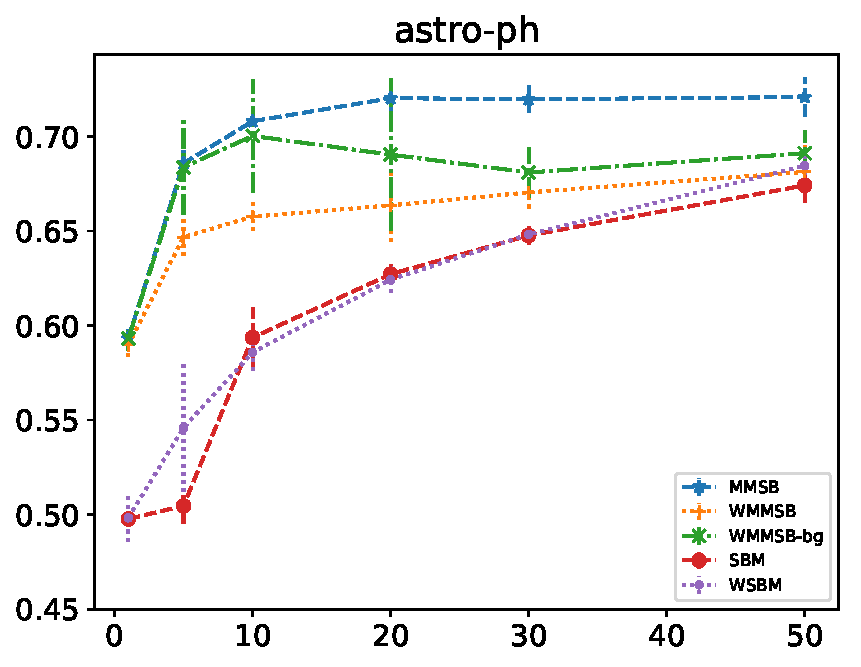
\includegraphics[width=0.32\textwidth]{fig/astro-ph__entropy@_roc_evo2}
\end{subfigure}
\begin{subfigure}
         \centering
      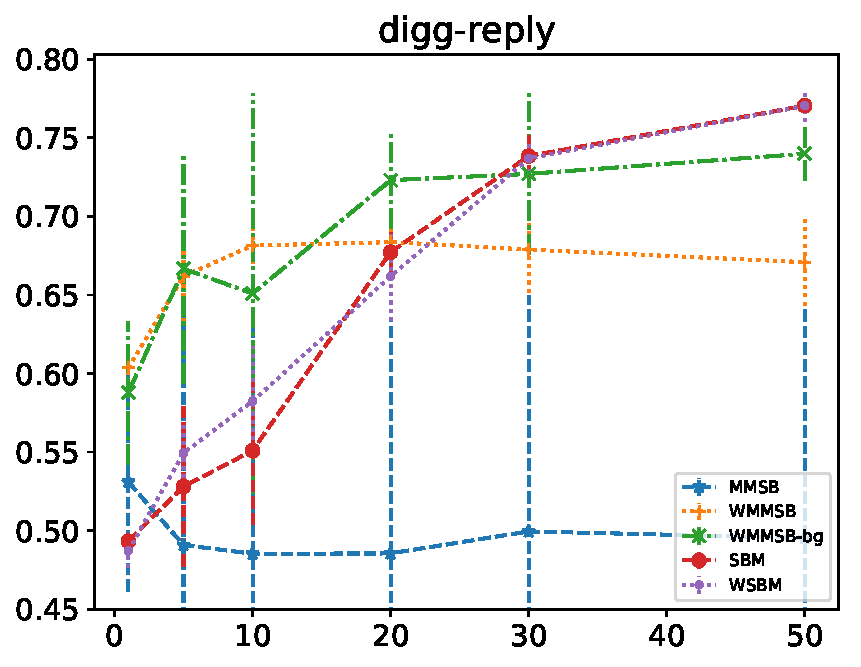
\includegraphics[width=0.32\textwidth]{fig/digg-reply__entropy@_roc_evo2}               
\end{subfigure}                                                                          
\begin{subfigure}                                                                        
         \centering                                                                      
      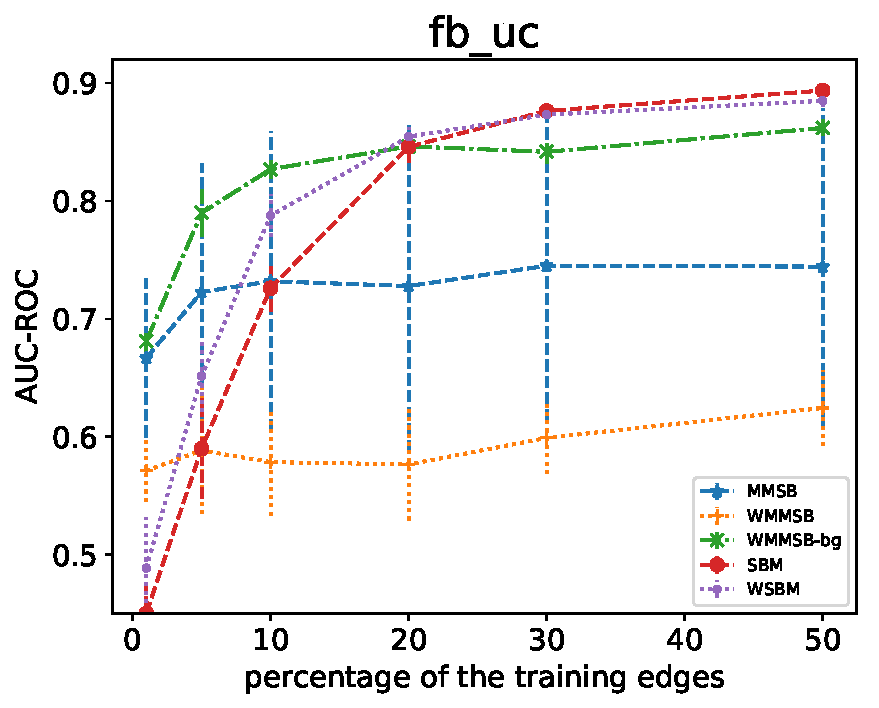
\includegraphics[width=0.32\textwidth]{fig/fb_uc__entropy@_roc_evo2}
\end{subfigure}                                                                          
\begin{subfigure}                                                                        
         \centering                                                                      
      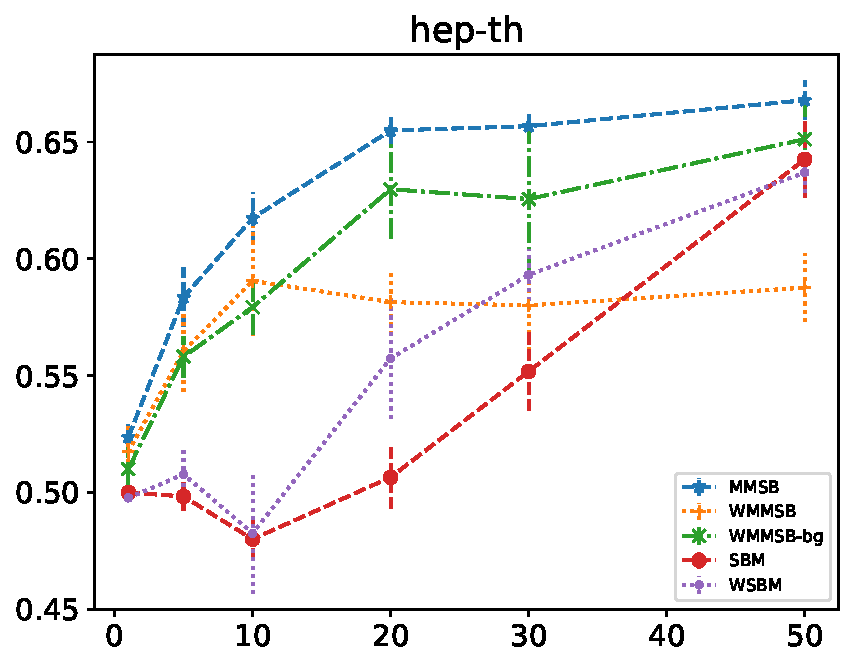
\includegraphics[width=0.32\textwidth]{fig/hep-th__entropy@_roc_evo2}
\end{subfigure}                                                                          
\begin{subfigure}
         \centering
      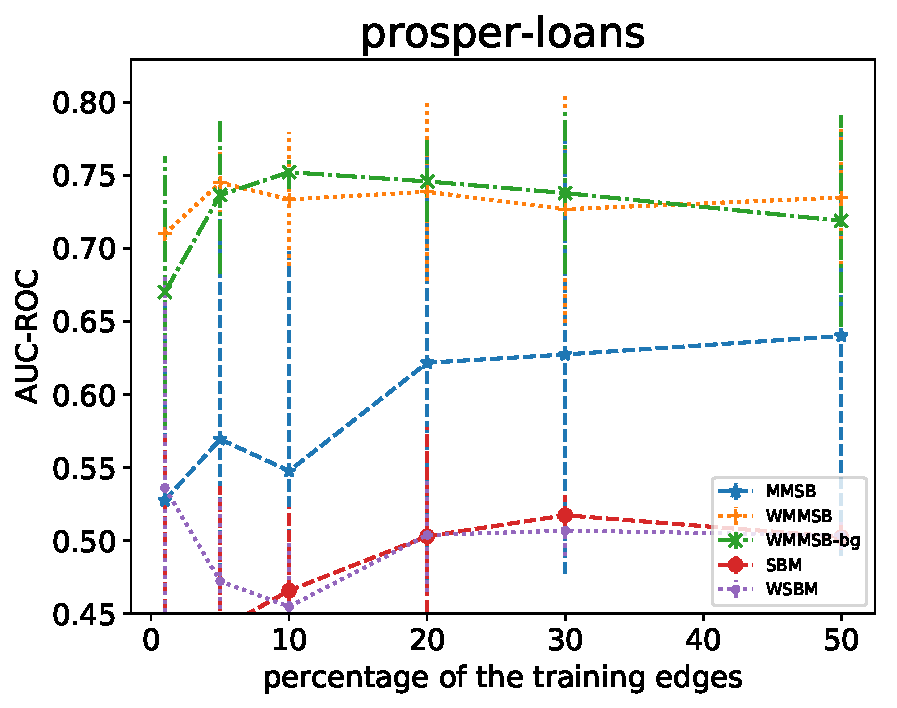
\includegraphics[width=0.32\textwidth]{fig/prosper-loans__entropy@_roc_evo2}
\end{subfigure}                                                             
\begin{subfigure}                                                           
         \centering                                                         
      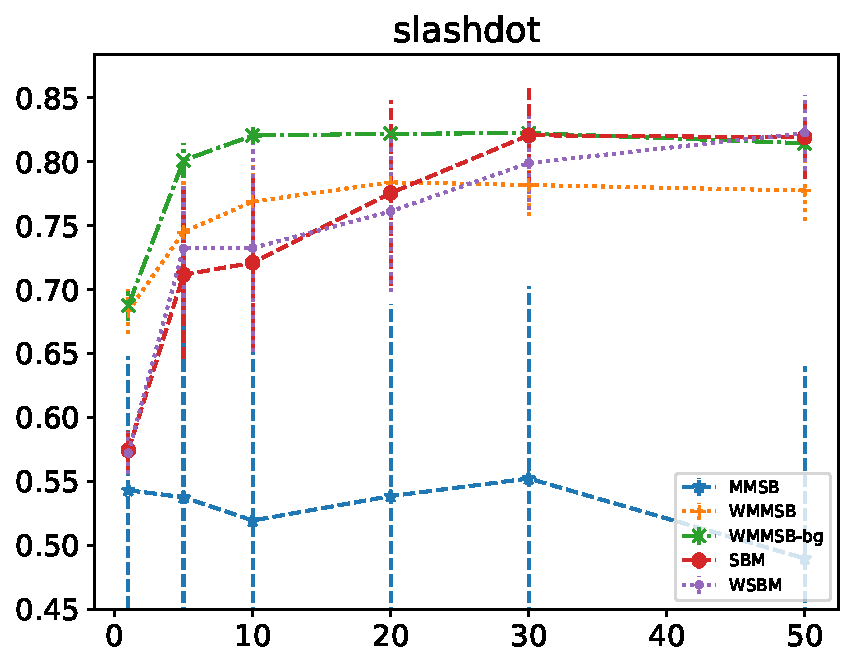
\includegraphics[width=0.32\textwidth]{fig/slashdot__entropy@_roc_evo2}
\end{subfigure}                                                             
\caption{Performance comparaison of models in terms of AUC-ROC score in function of the proportion of the observed edges used to train the models from 1 to 100 percent of the training set. Results are averaged on ten independant trials. Except for astro-ph and proper-loans where SBM and WSBM are not competitive, the curves cross each other at a specific proportion of training data under which MMSB, WMMSB and WMMSB-bg perfom better. }

